\documentclass{article}
\usepackage{graphicx}
\usepackage{amssymb}
\usepackage{amsmath}
\usepackage[colorlinks=true,linkcolor=blue,citecolor=green,urlcolor=red]{hyperref}

\begin{document}


\section*{Weekly Notes}

\subsection*{Date: 2023.10.13}

\subsubsection*{Concepts so far}
We have an unkown mapping $M: \mathbb{R}^n \rightarrow \mathbb{R}$. Even though the mapping is not known we are given the ability to observe the value of $M$ for any given point in $\mathbb{R}^n$.
Thus we can estimate this mapping by sampling $m$ datapoints from $\mathbb{R}^n$ and observing the corresponding values of $M$.
\\
We made two models $F$ and $G$ based on the gathered datapoints and/or other heuristics.
To see which model performs better we can calculate the R squared value for both the models and than perform a t-test to see if the difference in the R squared values is significant.
\\
\begin{figure}[h]
\centering
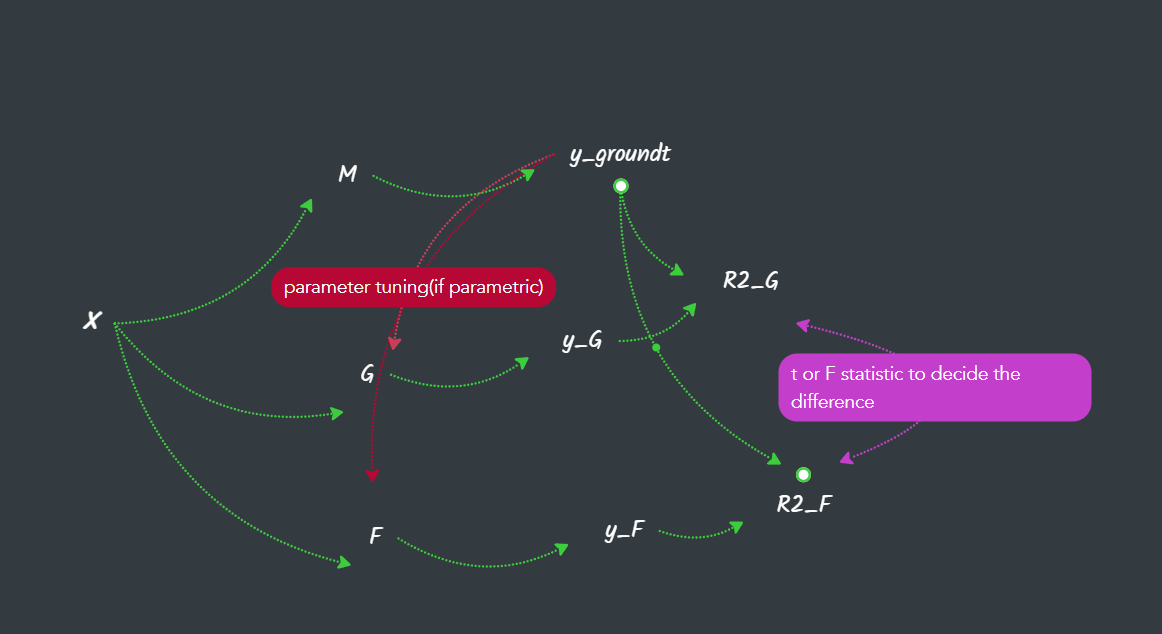
\includegraphics[width=1\textwidth]{sketch.png}
\caption{Sketch}
\end{figure}
\\
Suppose that $M=g(a)$, where $a=\sum_{i=1}^n x_i$, $g$ is a sigmoid function and each $x_i$ is sampled from distribution $D_i$.\\
Than if we omit $x_k$ from $a$ that is equivalent to adding negative noise from the distribution of $x_k$ to $a$.\\
$a_{-k}=\sum_{i=1, i\neq k}^n x_i$\\
$a_{-k}=a+\varepsilon$\\
where $\varepsilon \sim D_k$.\\\\\\\\\\\\
We can also try to quantify the effect of the noise added to $a$ on the value of $g(a)$ by taking the following integral.
\\
%equation for integral from -inf to inf 1/(1+e**-x)-1/(1+e**-(x+k))dx
$\int_{-\infty}^{\infty}(\frac{1}{1+e^{-(a+\varepsilon)}}-\frac{1}{1+e^{-a}}) da$
\\
% F(x) = ln(e**(x+11)-ln(e**(x)+1)
$F(x) = ln(e^{(a+\varepsilon)}-ln(e^{a}+1)$
\\
$\int_{-\infty}^{\infty}(\frac{1}{1+e^{-(a+\varepsilon)}}-\frac{1}{1+e^{-a}}) da=\varepsilon$\\
Where $\varepsilon$ is the sum of all errors between the value of $g(a)$ and $g(a_{-k})$ for all possible values of $a$ and $a_{-k}$.\\
This integral could also be taken for a finite range of $a$ values.\\
\subsubsection*{Problems}


Given,
\begin{align}
x_i \sim \mathrm{Bernauli}(p) \\
a = \gamma \sum_{i=1}^N (x_i-p)
\end{align}
a) What is the mean and variance of $a$ if $N$ is sufficiently large?
\begin{align}
\sum_{i=1}^N = N*p\\
a = \sum_{i=1}^N (x_i - p) = N*p - N*p\\
\mu_a (p, N) = 0\\
\sigma_a^2 (p, N) = 1/M * \sum_{j=1}^M (N*p-N*p-0)^2=0
\end{align}
b) What is the mean and variance of $a$ if $N$ is not large enough?
\begin{align}
    \sum_{i=1}^N = N*\hat{p}\\
    a_j = \sum_{i=1}^N (x_{i,j} - p) = N(\hat{p_j} - p)\\
    \mu_a (p, N) = N/M * \sum_{j=1}^M (\hat{p_j}-p)\\
    \sigma_a^2 (p, N) = 1/M * \sum_{j=1}^M (\hat{p}_j-p- N/M * \sum_{j=1}^M (\hat{p_j}-p))
\end{align}

For sufficiently large $M$, $\mu_a (p, N) = 0$ and $\sigma_a^2 (p, N) = \hat{p}_j-p$.




\end{document}
